\chapter{Specifikacija programske potpore}
		
	\section{Funkcionalni zahtjevi}
			\noindent \textbf{Dionici:}
			
	\begin{packed_enum}
				\item  Neregistrirani korisnik
				\item  Registrirani korisnik 
					\begin{packed_enum}
						
						\item  klijent
						\item  vlasnik kluba
						\item  trener
						\item administrator
				
					\end{packed_enum}

				\item Razvojni tim
				\item Asistenti
										
			\end{packed_enum}
			
			\noindent \textbf{Aktori i njihovi funkcionalni zahtjevi:}
			
			
			\begin{packed_enum}
				\item  \underbar{ Neregistrirani korisnik (inicijator) može:}
				
				\begin{packed_enum}
					\item pregledati na karti dostupne plesnjake i lokacije klubova
					\item odabrati profile klubova (ime kluba, kontakt telefon, email adresu, kratki opis)  i pregledati tipove plesa (naziv, kratki opis, slika i link na video primjer plesa) koje ti klubovi nude
					\item registrirati se, kreirati novi korisnički račun za klijenta za koji su mu potrebni korisničko ime, lozinka, ime, prezime, spol, datum rođenja, broj mobitela, email adresa i opcionalno opis plesnog iskustva i fotografija
					

					
				\end{packed_enum}
			
				\item  \underbar{Klijent (inicijator) može:}
				
				\begin{packed_enum}
					
					\item pregledavati i mijenjati osobne podatke
					\item izbrisati svoj korisnički račun
					\item  pregledati na karti tečajeve slobodne za upis 
					\item odabrati tečaj/grupu i dobiti prikaz relevantnih informacija (vrsta plesa, kalendar s terminima tečaja i lokacijama s dvoranama, ime i prezime te sliku trenera)
					\item kreirati novi korisnički račun za klub za koji su mu potrebni korisničko ime, lozinka, ime kluba, adresa sjedišta, telefon i email čime postaje vlasnik kluba
					\item poslati prijavu klubu da postane trener koja mora sadržavati motivacijsko pismo i potvrdu u pdf formatu da je osposobljen držati tečaj plesa
					\item pregledati aktivne prijave na tečaj/grupu kluba (informacije o treneru, skupu treninga kroz neko vrijeme, maksimalnom broju sudionika, opis s dodatnim informacijama o težini treninga, uvjetima treniranja i pravilima ponašanja) i prijaviti se

					
				\end{packed_enum}
			
			
				\item  \underbar{Vlasnik kluba (inicijator) može:}
				
				\begin{packed_enum}
					\item organizirati plesnjak uz odgovarajući opis (lokacija, naziv, opis i slika) – lokacija plesnjaka može biti na lokaciji kluba ili izvan nje 
					\item potvrditi klijenta kao trenera
					\item objaviti upise za tečaj/grupu s krajnjim rokom prijave i ograničenjem na dob i spol
					\item odabrati klijente koji se primaju na tečaj/grupu 
					\item naknadno mijenjati popis klijenata
					\item uređivati i brisati tečajeve/grupe
					\item pregledavati i mijenjati osobne podatke
					\item izbrisati svoj korisnički račun 

				\end{packed_enum}
			

			
				\item  \underbar{Trener (inicijator) može:}
				
				\begin{packed_enum}
					
					\item imati podstranicu na kojoj vidi popis tečajeva/grupa koje trenira
					\item vidjeti na kalendaru sve termine tečajeva/grupa koje vodi
					\item vidjeti opće informacije tečaja/grupe za kojeg je zadužen i popis klijenata koji bi trebali biti nazočni na tečaju/grupi

				\end{packed_enum}
			

			
				\item  \underbar{Administrator (inicijator) može:}
				
				\begin{packed_enum}
					
					\item može dodati, mijenjati i brisati plesove
					\item  odobriti prijavu kluba za korištenje aplikacije 
					\item pregledati popis svih klijenata i klubova
					\item uređivati korisničke račune

					
				\end{packed_enum}
			
			
				\item  \underbar{Baza podataka(sudionik) može:}
				
				\begin{packed_enum}
					
					\item pohranjuje sve podatke o korisnicima i njihovim ovlastima
					\item pohranjuje sve podatke o plesnim tečajevima i plesnjacima, njihovim lokacijama i opisima

					
				\end{packed_enum}
			\end{packed_enum}
			
			\eject 
			
			
				
			\subsection{Obrasci uporabe}
				
				\subsubsection{Opis obrazaca uporabe}

\noindent \underbar{\textbf{UC1 - Registracija korisnika}}
					\begin{packed_item}
	
						\item \textbf{Glavni sudionik: }Neregistrirani korisnik
						\item  \textbf{Cilj:} Stvoriti korisnički račun za pristup sustavu
						\item  \textbf{Sudionici:} Baza podataka
						\item  \textbf{Opis osnovnog tijeka:						
						}
						
						\item[] \begin{packed_enum}
	
							\item Korisnik odabire opciju za registraciju
							\item Korisnik unosi potrebne korisničke podatke
							\item Korisnik prima obavijest o uspješnoj registraciji
							
						\end{packed_enum}
						
						\item  \textbf{Opis mogućih odstupanja:}
						
						\item[] \begin{packed_item}
	
							\item[4.a] Odabir već zauzetog korisničkog imena i/ili e-maila, unos 
korisničkog podatka u nedozvoljenom formatu ili pružanje 
neispravnog e-maila

							\item[] \begin{packed_enum}
								
								\item Sustav obavještava korisnika o neuspjelom upisu i vraća 
ga na stranicu za registraciju
								\item Korisnik mijenja potrebne podatke te završava unos ili 
odustaje od registracije
																
							\end{packed_enum}
														
						\end{packed_item}
					\end{packed_item}
					
					\noindent \underbar{\textbf{UC2 - Registracija kluba}}
					\begin{packed_item}
	
						\item \textbf{Glavni sudionik: }Registrirani korisnik
						\item  \textbf{Cilj:} Stvoriti korisnički račun za klub
						\item  \textbf{Sudionici:} Baza podataka
						\item  \textbf{Opis osnovnog tijeka:						
						}
						
						\item[] \begin{packed_enum}
	
							\item Korisnik odabire opciju za registraciju kluba
							\item Korisnik unosi podatke vezano za klub
							\item Korisnik prima obavijest o uspješnoj registraciji
							
						\end{packed_enum}
						
						\item  \textbf{Opis mogućih odstupanja:}
						
						\item[] \begin{packed_item}
	
							\item[4.a] . Odabir već zauzetog korisničkog imena i/ili e-maila, unos korisničkog podatka u nedozvoljenom formatu ili pružanje neispravnog e-mail

							\item[] \begin{packed_enum}
								
								\item Sustav obavještava korisnika o neuspjelom upisu i vraća ga na stranicu za registraciju
								\item Korisnik mijenja potrebne podatke te završava unos ili 
odustaje od registracije
																
							\end{packed_enum}
														
						\end{packed_item}
					\end{packed_item}
					
					\noindent \underbar{\textbf{UC3 - Pregled klubova}}
					\begin{packed_item}
	
						\item \textbf{Glavni sudionik: }Neregistrirani korisnik
						\item  \textbf{Cilj:} Pregledati sve dostupne klubove
						\item  \textbf{Sudionici:} Baza podataka
						\item  \textbf{Opis osnovnog tijeka:						
						}
						
						\item[] \begin{packed_enum}
	
							\item Karta je prikazana prilikom učitavanja aplikacije
							\item Korisnik na karti odabire klub
							\item Prikazuju se tipovi plesa koje pojedini klub nudi
							\item Klubovi se mogu filtrirati po tipovima plesa za koje organizira 
tečaj
							\item Odabir filtra
							\item Prikazuju se filtrirani plesnjaci
							
						\end{packed_enum}
						
						
					\end{packed_item}
					
					\noindent \underbar{\textbf{UC4 -Pregled plesnjaka}}
					\begin{packed_item}
	
						\item \textbf{Glavni sudionik: }Neregistrirani korisnik
						\item  \textbf{Cilj:} Pregledati dostupne plesnjake
						\item  \textbf{Sudionici:} Baza podataka
						\item  \textbf{Opis osnovnog tijeka:						
						}
						
						\item[] \begin{packed_enum}
	
							\item Korisniku se na karti prikazuju dostupni plesnjaci 
							\item Dostupni plesnjaci se mogu filtrirati po:
							
							\item[] \begin{packed_enum}
								
								\item Tipu plesa
								\item Klubu koji ga organizira
								
							\end{packed_enum}
							
							\item Odabir filtra
							\item Prikazuju se filtrirani plesnjaci
						
						\end{packed_enum}	
						
					\end{packed_item}
					
					\noindent \underbar{\textbf{UC5 -Odabir kluba}}
					\begin{packed_item}
	
						\item \textbf{Glavni sudionik: }Neregistrirani korisnik
						\item  \textbf{Cilj:} Pretraga određenog kluba
						\item  \textbf{Sudionici:} Baza podataka
						\item  \textbf{Opis osnovnog tijeka:						
						}
						
						\item[] \begin{packed_enum}
	
							\item Pretraživanje kluba odvija se upisom osnovnih podataka o klubu  
							\item Prikazuju se podatci za traženi klub
							
						\end{packed_enum}	
						
					\end{packed_item}
					
					\noindent \underbar{\textbf{UC6 -Dodavanje plesa}}
					\begin{packed_item}
	
						\item \textbf{Glavni sudionik: }Administrator
						\item  \textbf{Cilj:} Dodati novi ples
						\item  \textbf{Preduvjet:} : Korisnik je registriran i dodijeljena su mu prava administratora
						\item  \textbf{Sudionici:} Baza podataka
						\item  \textbf{Opis osnovnog tijeka:						
						}
						
						\item[] \begin{packed_enum}
	
							\item Prikazuju se dostupni klubovi
							\item Odabire se klub kojem želi dodati određeni ples
							\item Unose se osnovni podatci o plesu
							\item Dodaje se novi ples u bazu podataka
							\item Ples postaje vidljiv unutar mogućih plesova za određeni klub
							
						\end{packed_enum}	
						
					\end{packed_item}
					
					\noindent \underbar{\textbf{UC7 - Izmjena plesa}}
					\begin{packed_item}
	
						\item \textbf{Glavni sudionik: }Administrator
						\item  \textbf{Cilj:} Izmjena postojećeg plesa
						\item  \textbf{Preduvjet:} : Korisnik je registriran i dodijeljena su mu prava administratora
						\item  \textbf{Sudionici:} Baza podataka
						\item  \textbf{Opis osnovnog tijeka:						
						}
						
						\item[] \begin{packed_enum}
	
							\item Prikazuju se dostupni klubovi 
							\item Administrator odabire klub
							\item Administrator odabire ples kojem želi izmijeniti određene 
podatke

							\item Promjene se upisuju u bazu podataka
							\item Izmijene postaju vidljive za odabrani ples
							
						\end{packed_enum}	
						
					\end{packed_item}
					
					\noindent \underbar{\textbf{UC8 - Brisanje plesa}}
					\begin{packed_item}
	
						\item \textbf{Glavni sudionik: }Administrator
						\item  \textbf{Cilj:} Brisanje postojećeg plesa
						\item  \textbf{Preduvjet:} : Korisnik je registriran i dodijeljena su mu prava administratora
						\item  \textbf{Sudionici:} Baza podataka
						\item  \textbf{Opis osnovnog tijeka:						
						}
						
						\item[] \begin{packed_enum}
	
							\item Prikazuju se dostupni klubovi 
							\item Odabir kluba
							\item Odabir plesa koji se želi obrisati
							\item Odabrani ples se uklanja iz baze podataka
							\item Obrisani ples nije više vidljiv u aplikaciji
							
						\end{packed_enum}	
						
					\end{packed_item}
					
					\noindent \underbar{\textbf{UC9 - Odobrenje prijave kluba}}
					\begin{packed_item}
	
						\item \textbf{Glavni sudionik: }Administrator
						\item  \textbf{Cilj:} Odobrenje prijave kluba za korištenje aplikacije 
						\item  \textbf{Preduvjet:} : Korisnik je registriran i dodijeljena su mu prava administratora
						\item  \textbf{Sudionici:} Baza podataka
						\item  \textbf{Opis osnovnog tijeka:						
						}
						
						\item[] \begin{packed_enum}
	
							\item Prikaz svih klubova koji traže pristup sustavu 
							\item Prijava se može odbiti ili prihvatiti
							\item U slučaju prihvaćanja, podatci za klub se spremaju u bazu podataka
							\item Klub je nakon toga vidljiv u aplikaciji
							
						\end{packed_enum}	
						
					\end{packed_item}
					
					\noindent \underbar{\textbf{UC10 - Pregled korisnika}}
					\begin{packed_item}
	
						\item \textbf{Glavni sudionik: }Administrator
						\item  \textbf{Cilj:} Pregledati registrirane korisnike
						\item  \textbf{Preduvjet:} : Korisnik je registriran i dodijeljena su mu prava administratora
						\item  \textbf{Sudionici:} Baza podataka
						\item  \textbf{Opis osnovnog tijeka:						
						}
						
						\item[] \begin{packed_enum}
	
							\item Administrator odabire opciju pregledavanja korisnika 
							\item Prikaže se lista svih ispravno registriranih korisnika s osobnim podatcima
							
						\end{packed_enum}	
						
					\end{packed_item}
					
					
					\noindent \underbar{\textbf{UC11 - Uređivanje korisničkih računa}}
					\begin{packed_item}
	
						\item \textbf{Glavni sudionik: }Administrator
						\item  \textbf{Cilj:} Uređivanje korisničkih računa
						\item  \textbf{Preduvjet:} : Korisnik je registriran i dodijeljena su mu prava administratora
						\item  \textbf{Sudionici:} Baza podataka
						\item  \textbf{Opis osnovnog tijeka:						
						}
						
						\item[] \begin{packed_enum}
	
							\item Odabir hoće li se urediti korisnički račun kluba ili klijenta 
							\item Odabir određenog korisničkog računa
							\item Prikazuju se podatci koje je moguće izmijeniti za određeni korisnički račun
 							\item Promjene se spremaju u bazu podataka
							
						\end{packed_enum}	
						
					\end{packed_item}					
					
										\noindent \underbar{\textbf{UC12 -Prijava u sustav}}
					\begin{packed_item}
	
						\item \textbf{Glavni sudionik: }Klijent
						\item  \textbf{Cilj:} Dobiti pristup korisničkom sučelju
						\item  \textbf{Sudionici:} Baza podataka
						\item  \textbf{Preduvjet:} Registracija
						\item  \textbf{Opis osnovnog tijeka:						
						}
						
						\item[] \begin{packed_enum}
	
							\item Unos korisničkog imena i lozinke
							\item Potvrda o ispravnosti unesenih podataka
							\item Pristup korisničkim funkcijama
							
						\end{packed_enum}
						
						\item  \textbf{Opis mogućih odstupanja:}
						
						\item[] \begin{packed_item}
	
							\item[2.a] Neispravno korisničko ime/lozinka
							\item[] \begin{packed_enum}
								
								\item Sustav obavještava korisnika o neuspješnoj prijavi i vraća ga na stranicu kao neregistriranog korisnika
																
							\end{packed_enum}
														
						\end{packed_item}
					\end{packed_item}

					\noindent \underbar{\textbf{UC13 -Pregled osobnih podataka}}
					\begin{packed_item}
	
						\item \textbf{Glavni sudionik: }Klijent
						\item  \textbf{Cilj:} Pregledati osobne podatke
						\item  \textbf{Sudionici:} Baza podataka
						\item  \textbf{Opis osnovnog tijeka:}
						
						\item[] \begin{packed_enum}
	
							\item Klijent odabire opciju prikaza osobnih podataka
							\item Aplikacija prikazuje osobne podatke
						\end{packed_enum}
						
					\end{packed_item}

					\noindent \underbar{\textbf{UC14 -Promjena osobnih podataka}}
					\begin{packed_item}
	
						\item \textbf{Glavni sudionik: }Klijent
						\item  \textbf{Cilj:} Promijeniti osobne podatke
						\item  \textbf{Sudionici:} Baza podataka
						\item  \textbf{Opis osnovnog tijeka:}
						
						\item[] \begin{packed_enum}
	
							\item Klijent odabire opciju promjene osobnih podataka
							\item Klijent mijenja svoje osobne podatke
							\item Klijent sprema promjene
							\item Ažuriraju se podatci u bazi podataka
						\end{packed_enum}
						
						\item  \textbf{Opis mogućih odstupanja:}
						
						\item[] \begin{packed_item}
	
							\item[2.a] Klijent promjeni osobne podatke, ali ne odabere opciju spremanja promjena
							\item[] \begin{packed_enum}
								
								\item Sustav obavještava klijenta da nije spremio podatke prije izlaska iz prozora
								
							\end{packed_enum}
							
						\end{packed_item}
					\end{packed_item}

					\noindent \underbar{\textbf{UC15 -Brisanje korisničkog računa}}
					\begin{packed_item}
	
						\item \textbf{Glavni sudionik: }Klijent
						\item  \textbf{Cilj:} Obrisati korisnički račun
						\item  \textbf{Sudionici:} Baza podataka
						\item  \textbf{Opis osnovnog tijeka:}
						
						\item[] \begin{packed_enum}
	
							\item Klijent odabire opciju prikaza osobnih podataka
							\item Otvara se stranica s osobnim podatcima klijenta
							\item Klijent briše račun
							\item Korisnički račun briše se iz baze podataka
							\item Otvara se stranica vidljiva neregistriranom korisniku
						\end{packed_enum}
						
					\end{packed_item}
					
					\noindent \underbar{\textbf{UC16 -Pregled tečajeva na karti slobodnih za upis}}
					\begin{packed_item}
	
						\item \textbf{Glavni sudionik: }Klijent
						\item  \textbf{Cilj:} Pregledati na karti tečajeve slobodne za upis
						\item  \textbf{Sudionici:} Baza podataka
						\item  \textbf{Opis osnovnog tijeka:						
						}
						
						\item[] \begin{packed_enum}
	
							\item Klijent odabire opciju prikaza slobodnih tečajeva na karti
							\item Otvara se stranica s kartom i prikazom tečajeva
							\item Ukoliko želi, klijent filtrira tečajeve prema željenom vremenu i vrsti plesa
						\end{packed_enum}
						
						\item  \textbf{Opis mogućih odstupanja:}
						
						\item[] \begin{packed_item}
	
							\item[2.a] Nema tečajeva slobodnih za upis 
							\item[] \begin{packed_enum}
								
								\item Sustav obavještava korisnika da trenutno nema tečajeva slobodnih za upis (općenito ili za određeno mjesto i/ili vrstu plesa)
																
							\end{packed_enum}
														
						\end{packed_item}
					\end{packed_item}
				
					\noindent \underbar{\textbf{UC17 -Odabir tečaja s karte}}
					\begin{packed_item}
	
						\item \textbf{Glavni sudionik: }Klijent
						\item  \textbf{Cilj:} Odabrati jedan od slobodnih tečajeva
						\item  \textbf{Sudionici:} Baza podataka
						\item  \textbf{Preduvjet:} Postoji slobodno mjesto za upis na tečaj
						\item  \textbf{Opis osnovnog tijeka:						
						}
						
						\item[] \begin{packed_enum}
	
							\item Klijent odabire željeni tečaj na karti
							\item Otvara se stranica s prikazom relevantnih informacija o tečaju
						\end{packed_enum}
					\end{packed_item}
				

					\noindent \underbar{\textbf{UC18 - Organizacija plesnjaka}}
					\begin{packed_item}
	
						\item \textbf{Glavni sudionik: }Vlasnik kluba
						\item  \textbf{Cilj:} Organizacija plesnjaka uz opis
						\item  \textbf{Sudionici:} Baza podataka
						\item  \textbf{Opis osnovnog tijeka:						
						}
						
						\item[] \begin{packed_enum}
	
							\item Vlasnik kluba odabirom pretraživanja dolazi na stranicu za unos novog plesnjaka
							\item Vlasnik kluba putem forme upisuje potrebne podatke o plesnjaku
							\item Vlasnik kluba potvrđuje izradu plesnjaka
							\item Potvrdom odabira podaci se spremaju u bazu podataka
						\end{packed_enum}
					\end{packed_item}

					\noindent \underbar{\textbf{UC19 - Objava upisa za tečaj}}
					\begin{packed_item}
	
						\item \textbf{Glavni sudionik: }Vlasnik kluba
						\item  \textbf{Cilj:} Upis klijenata na tečaj
						\item  \textbf{Sudionici:} Baza podataka
						\item  \textbf{Opis osnovnog tijeka:}
						
						\item[] \begin{packed_enum}
	
							\item Vlasnik kluba na izborniku odabire opciju za objavu novog tečaja
							\item Vlasnik kluba treba unijeti potrebne podatke o tečaju
							\item Potvrdnim odabirom podaci o tečaju se spremaju u bazu podataka i postaju dostupni svima na izbor
						\end{packed_enum}
						
						\item  \textbf{Opis mogućih odstupanja:}
						
						\item[] \begin{packed_item}
	
							\item[2.a] Vlasnik kluba nije ispunio sve podatke
							\item[] \begin{packed_enum}
								
								\item Stranica vraća vlasnika kluba natrag te traži od njega unos svih potrebnih podataka
								
							\end{packed_enum}							
						\end{packed_item}
					\end{packed_item}

					\noindent \underbar{\textbf{UC20 - Odabir klijenata za tečaj}}
					\begin{packed_item}
	
						\item \textbf{Glavni sudionik: }Vlasnik kluba
						\item  \textbf{Cilj:} Popuna kvote za tečaj
						\item  \textbf{Sudionici:} Baza podataka
						\item  \textbf{Preduvjet:} Postoje prijave za tečaj
						\item  \textbf{Opis osnovnog tijeka:}
						
						\item[] \begin{packed_enum}
	
							\item Vlasnik kluba dobiva popis klijenata koji su se prijavili na tečaj
							\item Vlasnik kluba bira klijente prema ograničenjima koja su postavili
							\item Klikom na potvrdu odabira lista klijenata za tečaj je završena i sprema se u bazu podataka
						\end{packed_enum}
					\end{packed_item}

					\noindent \underbar{\textbf{UC21 - Mijenjanje popisa klijenata}}
					\begin{packed_item}
	
						\item \textbf{Glavni sudionik: }Vlasnik kluba
						\item  \textbf{Cilj:} Promjena popisa klijenata primljenih na tečaj
						\item  \textbf{Sudionici:} Baza podataka
						\item  \textbf{Preduvjet:} Postoji popis odabranih klijenata za tečaj
						\item  \textbf{Opis osnovnog tijeka:}
						
						\item[] \begin{packed_enum}
	
							\item Vlasnik kluba iz baze podataka uzima popis trenutnih klijenata na tečaju
							\item Vlasnik kluba miče klijente sa popisa ili dodaje nove, ovisno o potrebi
							\item Promijenjeni popis sprema se natrag u bazu podataka
						\end{packed_enum}
					\end{packed_item}

					\noindent \underbar{\textbf{UC22 - Uređivanje tečaja}}
					\begin{packed_item}
	
						\item \textbf{Glavni sudionik: }Vlasnik kluba
						\item  \textbf{Cilj:} Promjena uvjeta nekog tečaja
						\item  \textbf{Sudionici:} Baza podataka
						\item  \textbf{Preduvjet:} Tečaj postoji i objavljen je
						\item  \textbf{Opis osnovnog tijeka:}
						
						\item[] \begin{packed_enum}
	
							\item Vlasnik kluba na izborniku odabire promjenu tečaja
							\item Iz baze podataka se dopremaju podaci o tečaju
							\item Vlasnik kluba mijenja prethodno određene karakteristike
							\item Vlasnik kluba sprema podatke nakon što je gotov sa izmjenom
							\item Promijenjene karakteristike se spremaju u bazu podataka
						\end{packed_enum}
						
						\item  \textbf{Opis mogućih odstupanja:}
						
						\item[] \begin{packed_item}
	
							\item[2.a] Vlasnik kluba unio je neispravne podatke
							\item[] \begin{packed_enum}
								
								\item Stranica od njega zahtjeva da unese ispravne podatke
								
							\end{packed_enum}
						\end{packed_item}
					\end{packed_item}

					\noindent \underbar{\textbf{UC23 - Brisanje tečaja}}
					\begin{packed_item}
	
						\item \textbf{Glavni sudionik: }Vlasnik kluba
						\item  \textbf{Cilj:} Obrisati tečaj
						\item  \textbf{Sudionici:} Baza podataka
						\item  \textbf{Preduvjet:} Tečaj postoji
						\item  \textbf{Opis osnovnog tijeka:}
						
						\item[] \begin{packed_enum}
	
							\item Vlasnik kluba odabire opciju brisanja tečaja
							\item Tečaj se briše iz baze podataka i nije više dostupan
						\end{packed_enum}
						
					\end{packed_item}

					
					\noindent \underbar{\textbf{UC24 -Slanje prijave za trenera}}
					\begin{packed_item}
	
						\item \textbf{Glavni sudionik: }Klijent
						\item  \textbf{Cilj:} Klijent šalje prijavu određenom klubu kako bi postao njihov trener
						\item  \textbf{Sudionici:} Baza podataka
						\item  \textbf{Opis osnovnog tijeka:						
						}
						
						\item[] \begin{packed_enum}
	
							\item Klijent odabire određeni klub
							\item Klijent odabire opciju slanja prijave za trenera
							\item Otvara se prozor sa formom za unos osobnih podataka i datoteka – motivacijsko pismo i potvrda o sposobnosti vođenja tečaja
							\item Klijent unosi podatke i potvrđuje slanje
							\item Podaci se pohranjuju u bazu podataka
							\item Klubu se aplikaciji prikazuje nova prijava
						\end{packed_enum}
						
						\item  \textbf{Opis mogućih odstupanja:}
						
						\item[] \begin{packed_item}
	
							\item[4.a] Podaci u formi imaju krivi format ili nisu ispunjena obavezna polja
							\item[] \begin{packed_enum}
								
								\item Aplikacija obavještava klijenta da unese ispravne i obavezne podatke
																
							\end{packed_enum}
														
						\end{packed_item}
					\end{packed_item}
					
					\noindent \underbar{\textbf{UC25 – Potvrda prijave za trenera}}
					\begin{packed_item}
	
						\item \textbf{Glavni sudionik: }Klub
						\item  \textbf{Cilj:} Klijent postaje trener u određenom klubu
						\item  \textbf{Sudionici:} Baza podataka
						\item  \textbf{Preduvjet:} Klijent poslao prijavu za trenera
						\item  \textbf{Opis osnovnog tijeka:}
						
						\item[] \begin{packed_enum}
	
							\item Klub odabire prijavu od određenog klijenta
							\item Klub potvrđuje prijavu
							\item Klijentu se dodjeljuju ovlasti trenera
							\item Prijava se označava kao obrađena
						\end{packed_enum}
							
						\end{packed_item}
					\end{packed_item}
					
					\noindent \underbar{\textbf{UC26 - Odbijanje prijave za trenera}}
					\begin{packed_item}
	
						\item \textbf{Glavni sudionik: }Klub
						\item  \textbf{Cilj:} Klijentu se odbija poslana prijava za trenera
						\item  \textbf{Sudionici:} Baza podataka
						\item  \textbf{Preduvjet:} Klijent poslao prijavu za trenera
						\item  \textbf{Opis osnovnog tijeka:}
						
						\item[] \begin{packed_enum}
	
							\item Klub odabire prijavu od određenog klijenta
$>$
							\item Klub odbija određenog klijentaa
							\item Prijava se označava kao obrađena
						\end{packed_enum}
						\end{packed_item}
					\end{packed_item}
					
					\noindent \underbar{\textbf{UC27 – Pregled vođenih tečajeva}}
					\begin{packed_item}
	
						\item \textbf{Glavni sudionik: }Trener
						\item  \textbf{Cilj:} Vidjeti popis tečajeva koje vodi
						\item  \textbf{Sudionici:} Baza podataka
						\item  \textbf{Preduvjet:} Trener vodi tečaj za određeni klub
						\item  \textbf{Opis osnovnog tijeka:}
						
						\item[] \begin{packed_enum}
	
							\item Trener odabire opciju za prikaz svojih tečajeva
							\item Aplikacije prikazuje popis tečajeva koje trener vodi
							\item Trener odabire određeni tečaj
							\item Prikazuje se naziv tečaja sa opisom i nužnim informacijama o tečaju
						\end{packed_enum}
						
						\end{packed_item}
					\end{packed_item}
				
				
					\noindent \underbar{\textbf{UC28 - Pregled kalendara s vođenim terminima}}
					\begin{packed_item}
	
						\item \textbf{Glavni sudionik: }Trener
						\item  \textbf{Cilj:} Vidjeti kalendar s popisom treninga koje vodi određenog dana i sata
						\item  \textbf{Sudionici:} Baza podataka
						\item  \textbf{Opis osnovnog tijeka:}
						
						\item[] \begin{packed_enum}
	
							\item Trener odabire opciju za prikaz svojih vođenih termina
							\item Prikazuje se kalendar s označenim terminima kada vodi tečaj
						\end{packed_enum}
						\end{packed_item}
					\end{packed_item}
					
					\noindent \underbar{\textbf{UC29 - Pregled polaznika }}
					\begin{packed_item}
	
						\item \textbf{Glavni sudionik: }Trener
						\item  \textbf{Cilj:} Vidjeti popis nazočnih sudionika na tečaju
						\item  \textbf{Sudionici:} Baza podataka
						\item  \textbf{Preduvjet:} Trener vodi odabrani tečaj
						\item  \textbf{Opis osnovnog tijeka:}
						
						\item[] \begin{packed_enum}
	
							\item Trener odabire određeni tečaja iz popisa tečajeva
							\item Prikazuje se popis sudionika na tečaju s osnovnim osobnim podacima
						\end{packed_enum}
						
						\end{packed_item}
					\end{packed_item}

					\noindent \underbar{\textbf{UC30 - Pregled aktivnih prijava na tečaj kluba }}
					\begin{packed_item}
	
						\item \textbf{Glavni sudionik: }Klijent
						\item  \textbf{Cilj:} Pregledati aktivne prijave na tečajeve od klubova
						\item  \textbf{Sudionici:} Baza podataka
						\item  \textbf{Preduvjet:} Postoje aktivne prijave na tečajeve
						\item  \textbf{Opis osnovnog tijeka:}
						
						\item[] \begin{packed_enum}
	
							\item Klijent odabire opciju prikaza aktivnih prijava na tečajeve
							\item Prikazuje se stranica koja sadrži relevantne informacije o treninzima
						\end{packed_enum}
						
						\end{packed_item}
					\end{packed_item}

					\noindent \underbar{\textbf{UC31 -Prijava na tečaj kluba }}
					\begin{packed_item}
	
						\item \textbf{Glavni sudionik: }Klijent
						\item  \textbf{Cilj:} Prijaviti se na tečaj kluba
						\item  \textbf{Sudionici:} Baza podataka
						\item  \textbf{Preduvjet:} Postoje aktivne prijave na tečaj
						\item  \textbf{Opis osnovnog tijeka:}
						
						\item[] \begin{packed_enum}
	
							\item Klijent odabire opciju prikaza aktivnih prijava na tečajeve
							\item Prikazuje se stranica koja sadrži relevantne informacije o treninzima
							\item Klijent odabire opciju prijave na tečaj
							\item Klijent potvrđuje svoj odabir
							\item Prijava klijenta sprema se u bazu podataka te na listu prijavljenih kluba
						\end{packed_enum}
						
						\end{packed_item}
					\end{packed_item}
					
					
				\subsubsection{Dijagrami obrazaca uporabe}
				\eject		
				
				\begin{figure}[H]
			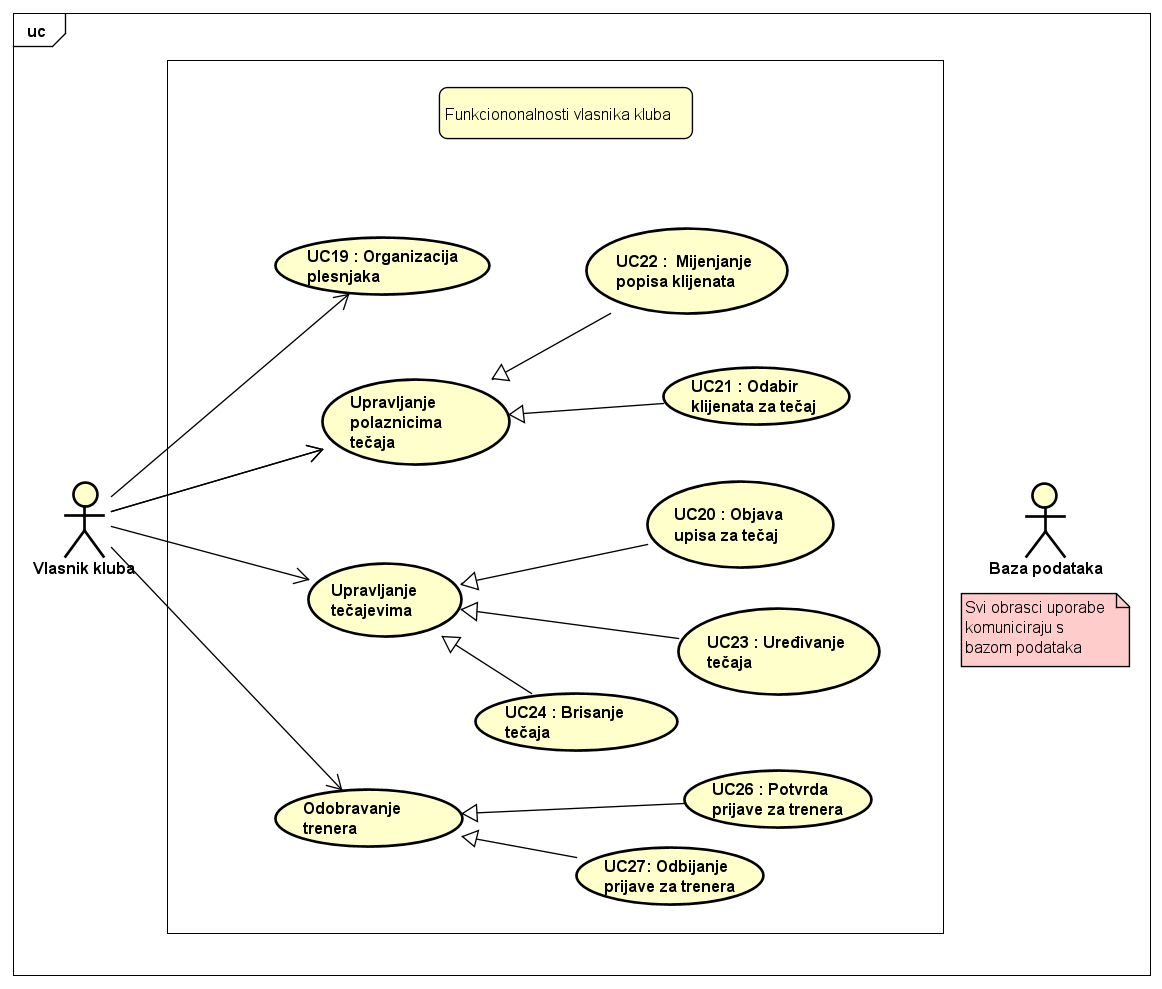
\includegraphics[scale=0.4]{slike/UC_klub.PNG} %veličina u odnosu na širinu linije
			\caption{Dijagram obrasca uporabe, funkcionalnost vlasnika kluba.}
			\label{fig:UC_klub} %label mora biti drugaciji za svaku sliku
		\end{figure}
		
		\begin{figure}[H]
			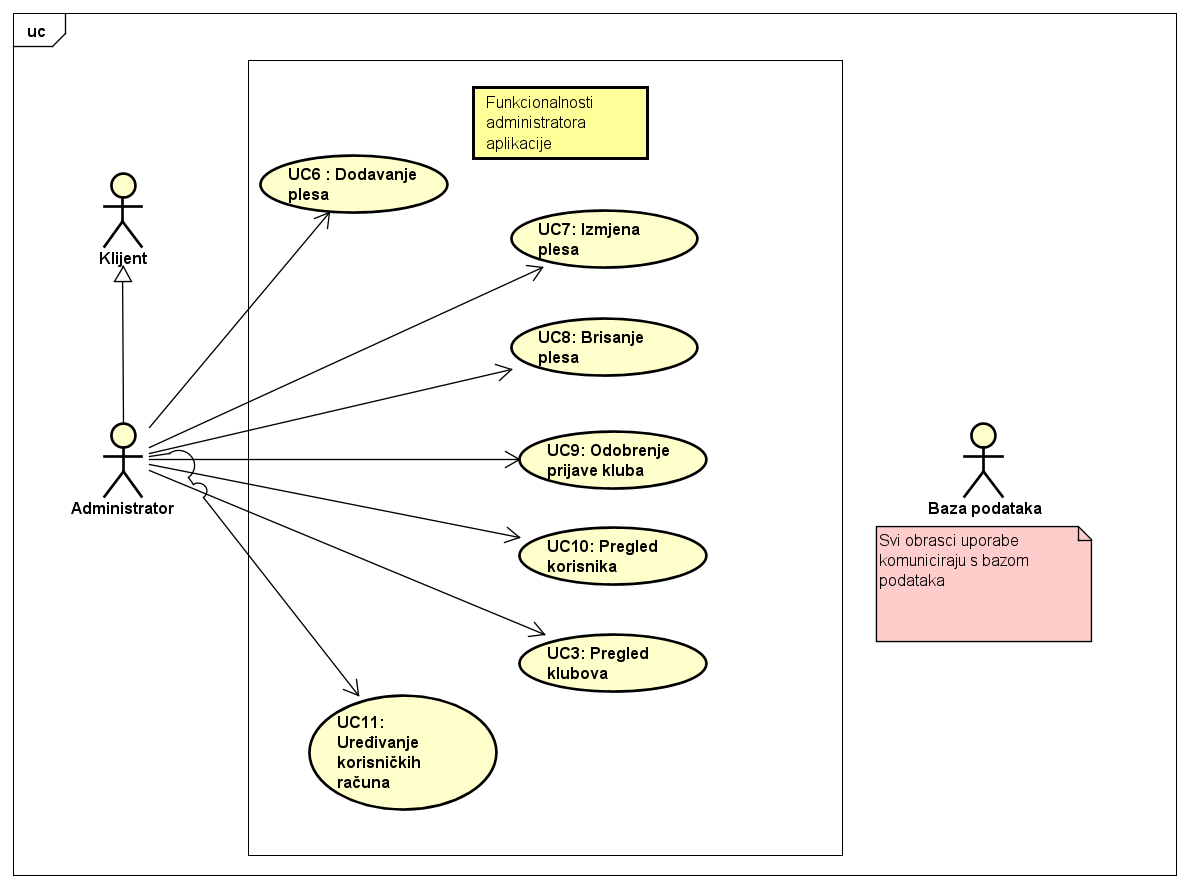
\includegraphics[scale=0.4]{slike/UC_admin.PNG} %veličina u odnosu na širinu linije
			\caption{Dijagram obrasca uporabe, funkcionalnost administratora.}
			\label{fig:UC_admin} %label mora biti drugaciji za svaku sliku
		\end{figure}

		\begin{figure}[H]
			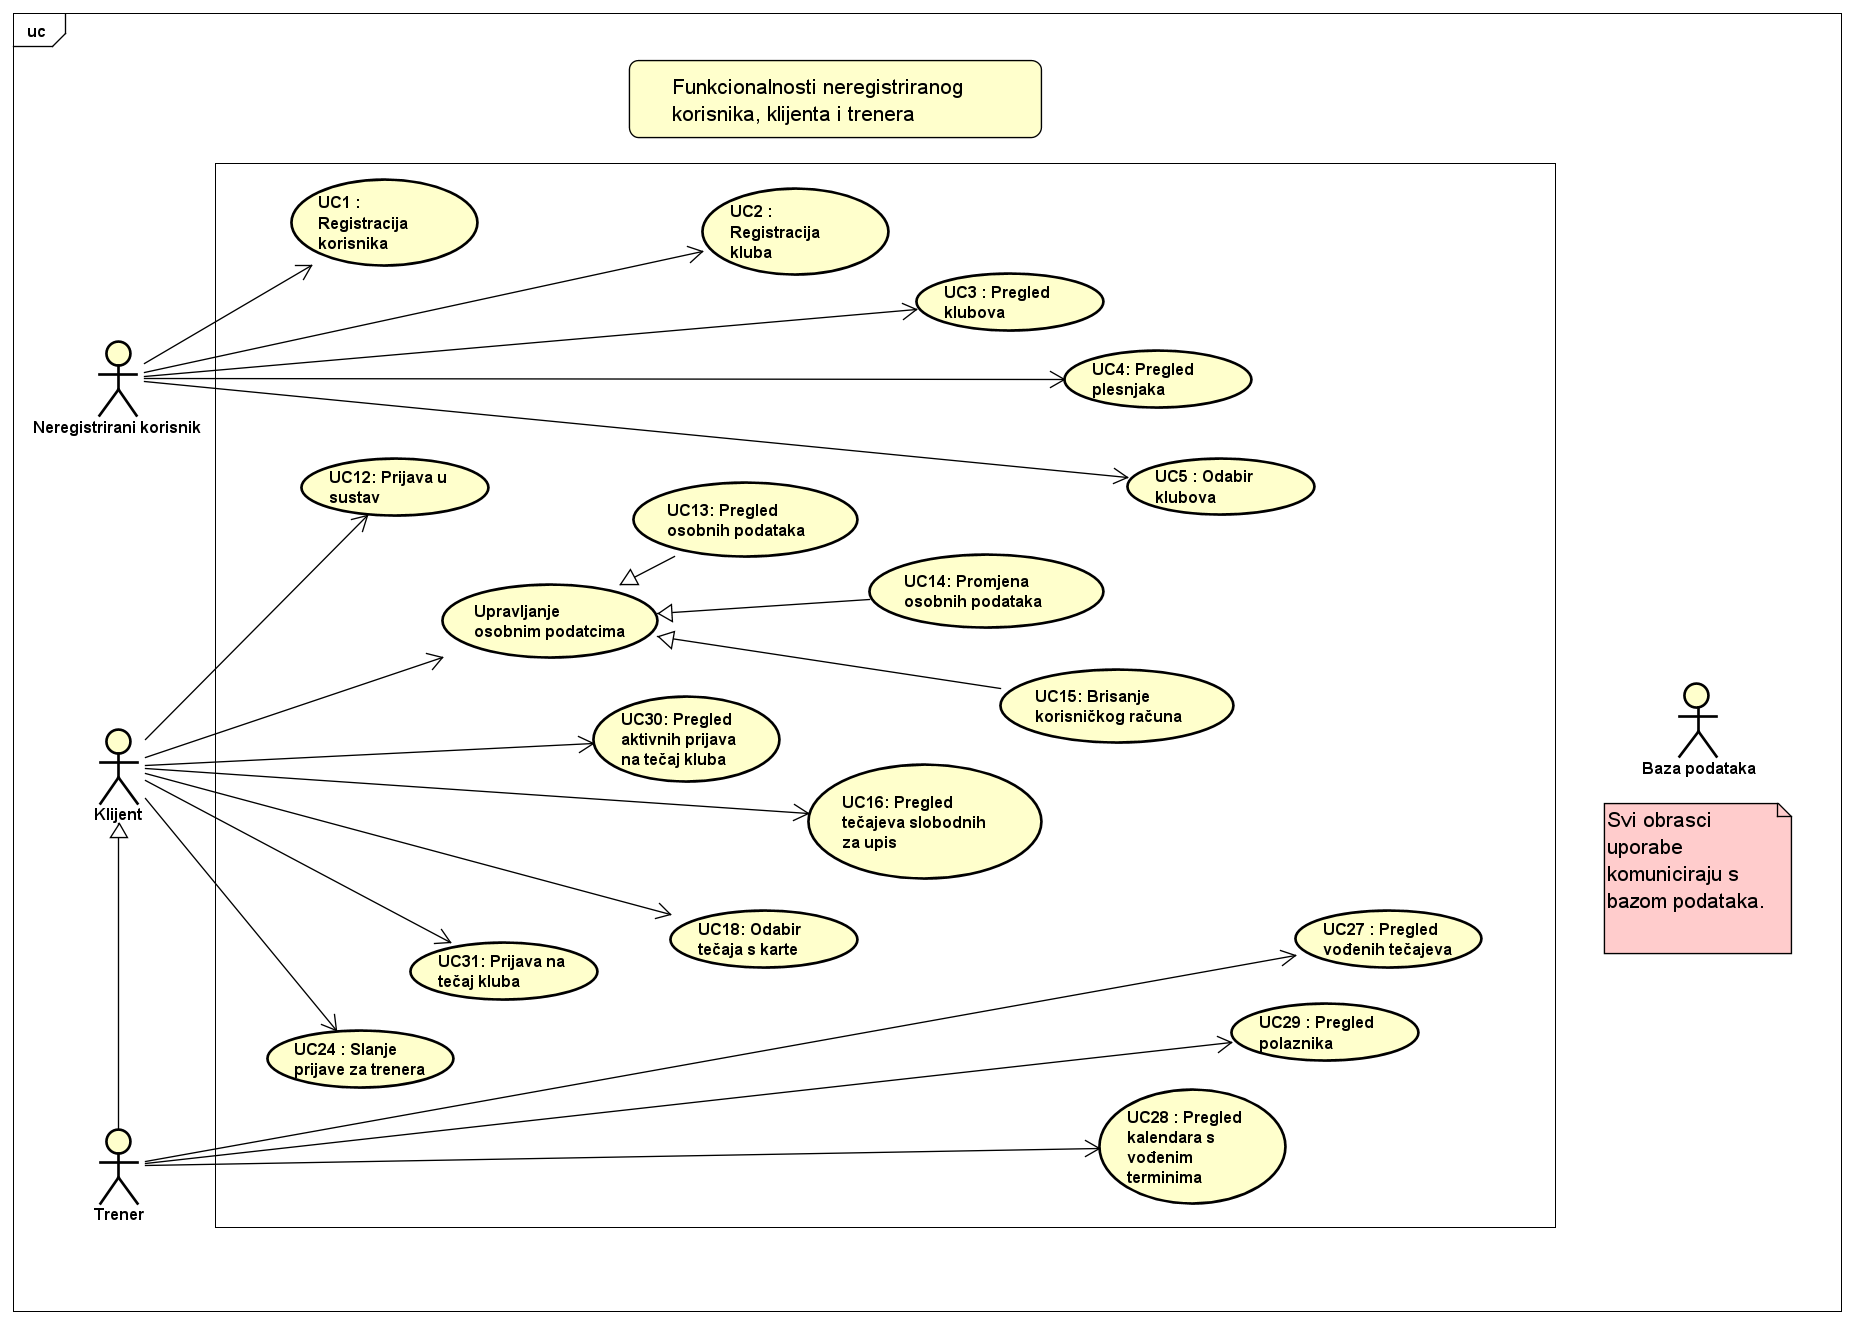
\includegraphics[scale=0.3]{slike/UC_Admin_client_unregistered.PNG} %veličina u odnosu na širinu linije
			\caption{Dijagram obrasca uporabe, funkcionalnost neregistriranog korisnika, klijenta i trenera.}
			\label{fig:UC_klijent_trener_neregistrirani} %label mora biti drugaciji za svaku sliku
		\end{figure}
		
		
				
			\subsection{Sekvencijski dijagrami}
				\noindent \textbf {Obrasci uporabe – UC25, UC26, UC27, UC28, UC29, UC30 - Slanje prijave za trenera, Potvrda prijave za trenera, Odbijanje prijave za trenera, Pregled vođenih tečajeva, Pregled kalendara s vođenim terminima, Pregled polaznika}
Klijent odabire opciju prijave trenera na poslužitelju, a poslužitelj mu vraća formu koju je potrebno ispuniti. Klijent unosi podatke potrebne za prijavu kako bi postao trener, poslužitelj provjerava ispravnost podataka te ih, ako su ispravni, pohranjuje u bazu podataka kao novu prijavu. Vlasnik kluba ima mogućnost pregleda svih prijava za trenere, odabire pregled prijava na poslužitelju, poslužitelj dohvaća podatke iz baze podataka te ih prikazuje vlasniku kluba. Novu prijavu za trenera vlasnik kluba može potvrditi ili odbiti. U slučaju ispunjenih kriterija vlasnik kluba odabire opciju potvrde trenera na poslužitelju, poslužitelj generira objekt novog trenera i unosi podatke o novom treneru u bazu podataka te vraća potvrdu o obavljenim akcijama. Ukoliko kriteriji nisu zadovoljeni, vlasnik kluba odabire opciju odbijanja nove prijave na poslužitelju, poslužitelj mijenja podatke vezane uz tu prijavu u bazi podataka te šalje potvrdu o obavljanju navedenih promjena.  Klijent koji ima potvrđenu ulogu trenera može na poslužitelju zatražiti pregled vođenih tečajeva, poslužitelj dohvaća podatke o njegovim tečajevima iz baze podataka te mu ih prikazuje. Također, može vidjeti prikaz kalendara s terminima tečajeva koje vodi, šalje zahtjev na poslužitelj, poslužitelj dohvaća podatke iz baze podataka, generira kalendar s dohvaćeni podacima te ih prikazuje treneru. Treneru je na poslužitelju omogućen i odabir pregleda popisa klijenata nazočnih na pojedinom terminu, poslužitelj u tom slučaju dohvaća podatke iz baze podataka, generira odgovarajući popis i prikazuje ih treneru. 
				
				%unos slike
		\begin{figure}[H]
			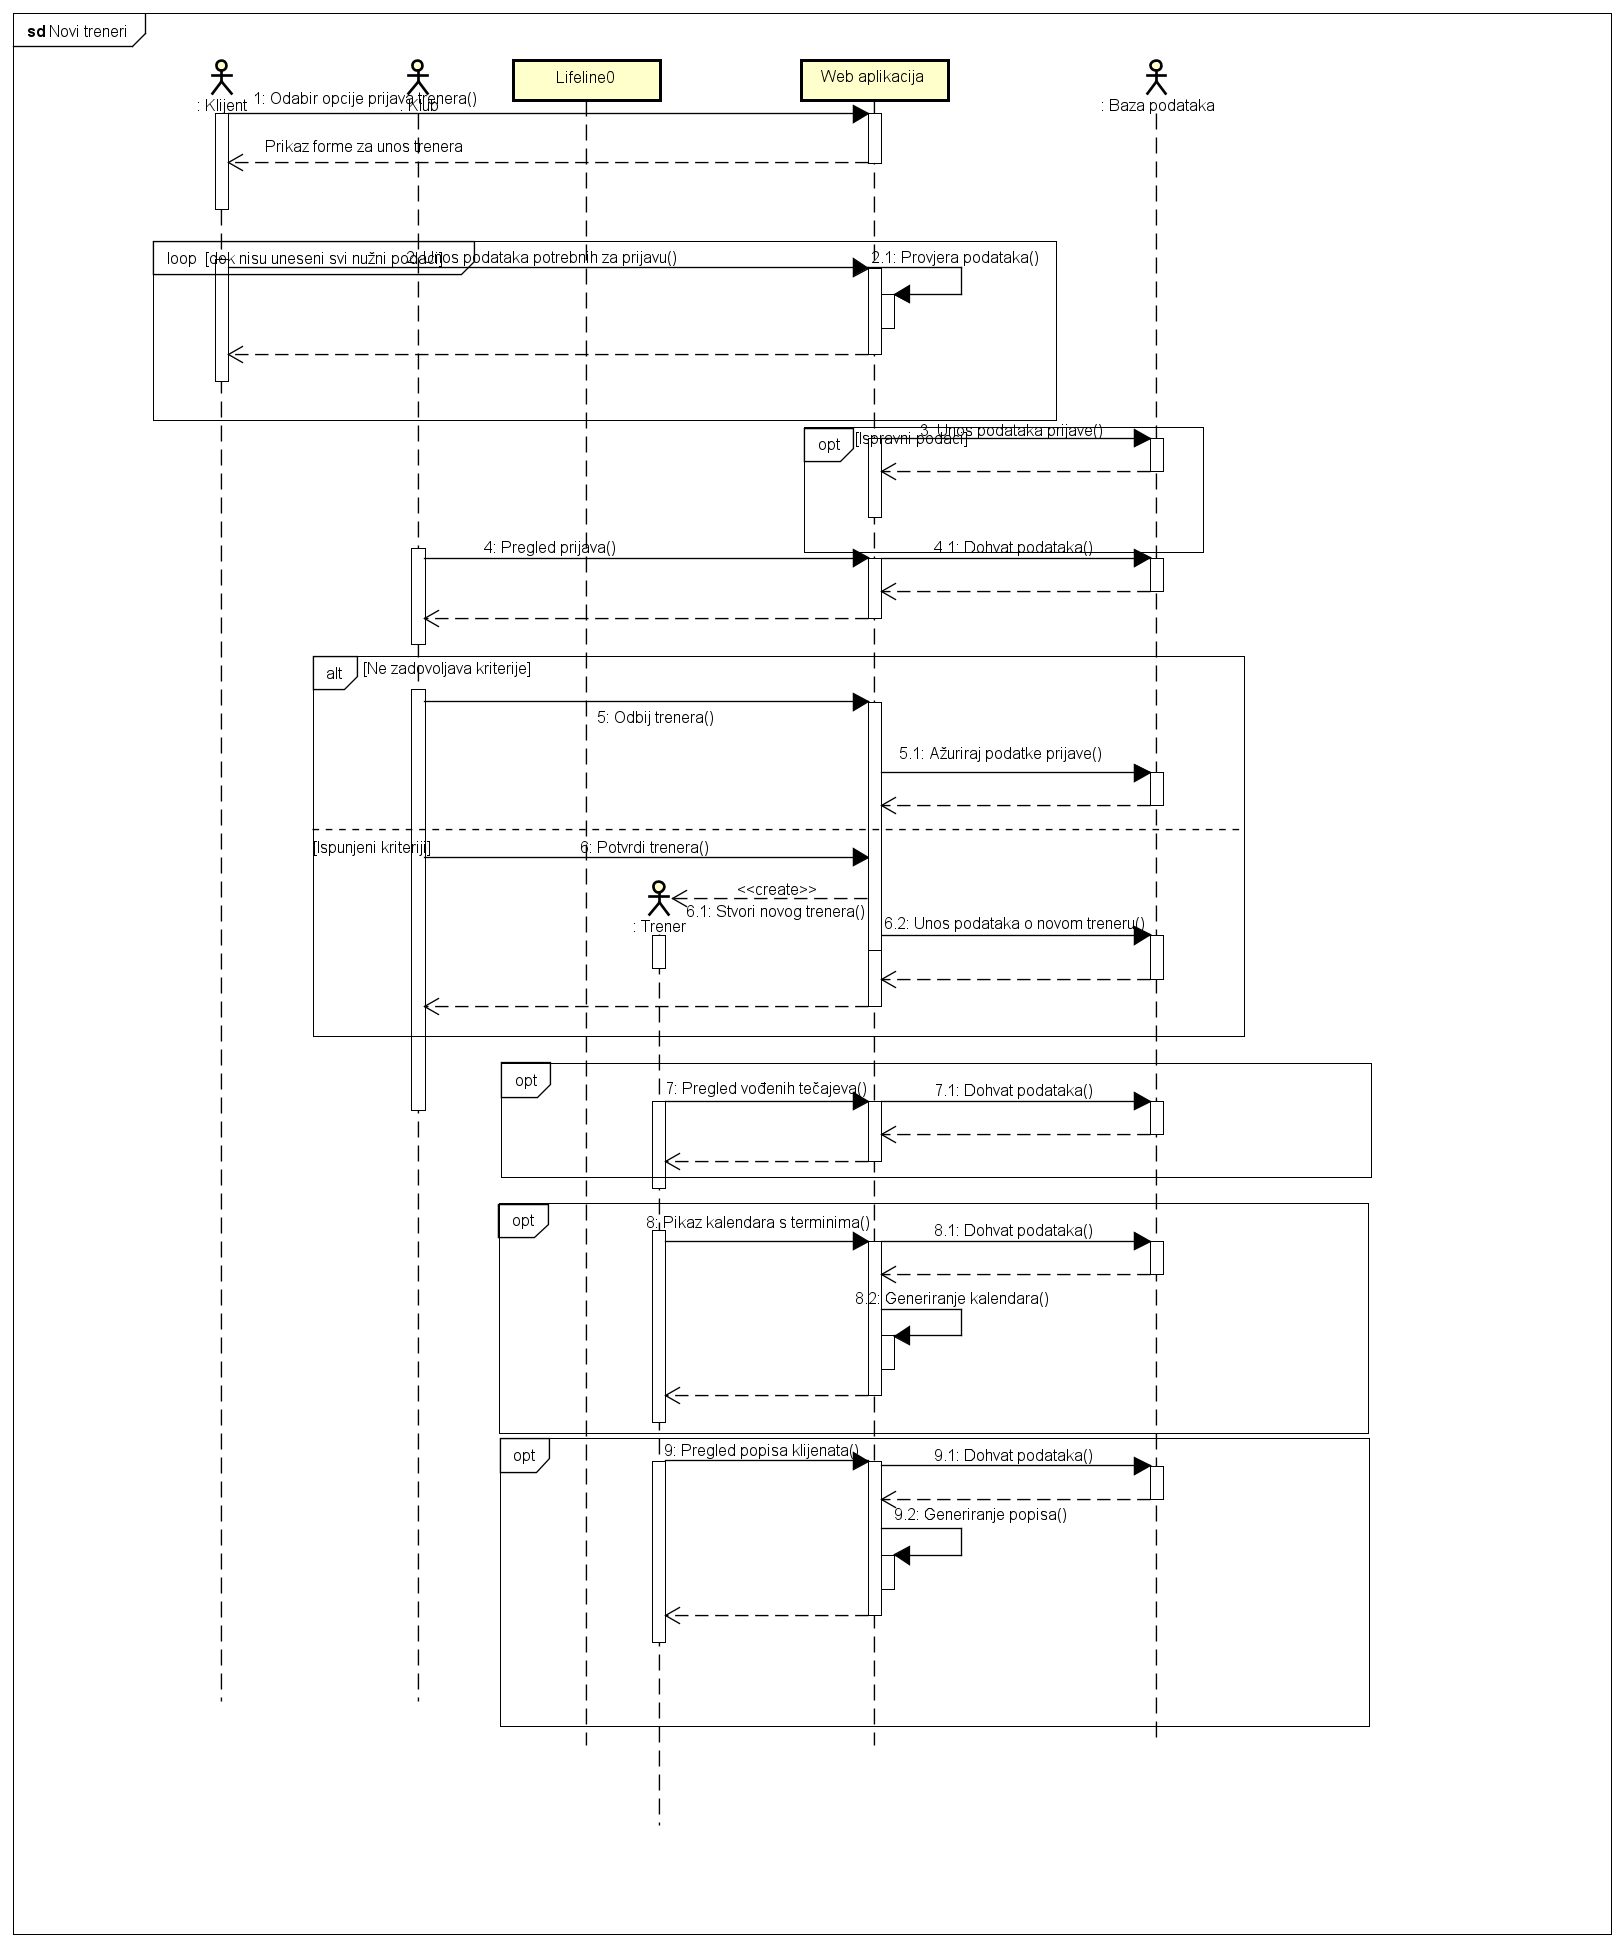
\includegraphics[scale=0.4]{slike/SD-prijavaTrenera.PNG} %veličina slike u odnosu na originalnu datoteku i pozicija slike
			\centering
			\caption{Sekvencijski dijagram - Prijava trenera i njegove funkcionalnosti}
			\label{fig:trener}
		\end{figure}
		
				\noindent \textbf {Obrasci uporabe - UC17, UC20, UC21, UC22, UC32 - Objava upisa na tečaj, pregled tečajeva, prijava na tečaj, odabir klijenata za tečaj i mijenjanje popisa klijenata} 
Vlasnik kluba šalje zahtjev za izradu tečaja, nakon čega mu poslužitelj vraća formu za upis podataka o tečaju. Poslužitelj zatim podatke o tečaju upisuje u bazu. Klijent šalje zahtjev za pregledom tečajeva. Poslužitelj iz baze dohvaća podatke o tečajevima i prikazuje ih klijentu. Klijent odabire jedan tečaj i prijavi se na njega, nakon čega poslužitelj vrši provjeru ispravnosti. Ako je klijent unio ispravne podatke, poslužitelj u bazu unosi podatke o prijavi i vraća korisniku povratnu informaciju o uspješnosti prijave. Vlasnik kluba šalje zahtjev poslužitelju za pregled prijava. Poslužitelj dohvaća prijave iz baze i šalje ih vlasniku kluba na pregled. Vlasnik kluba zatim odlučuje o potencijalnoj potvrdi klijenta na tečaj, nakon čega poslužitelj ažurira status prijave u bazi podataka. Vlasnik kluba po volji može izmijeniti popis klijenata za tečaj, za što prvo mora poslati zahtjev poslužitelju za dohvat podataka o tečaju. Poslužitelj dohvaća podatke iz baze i šalje ih vlasniku kluba. Vlasnik kluba zatim vrši izmjene i potvrđuje ih, nakon čega poslužitelj ažurira podatke o tečaju u bazi.

		\begin{figure}[H]
			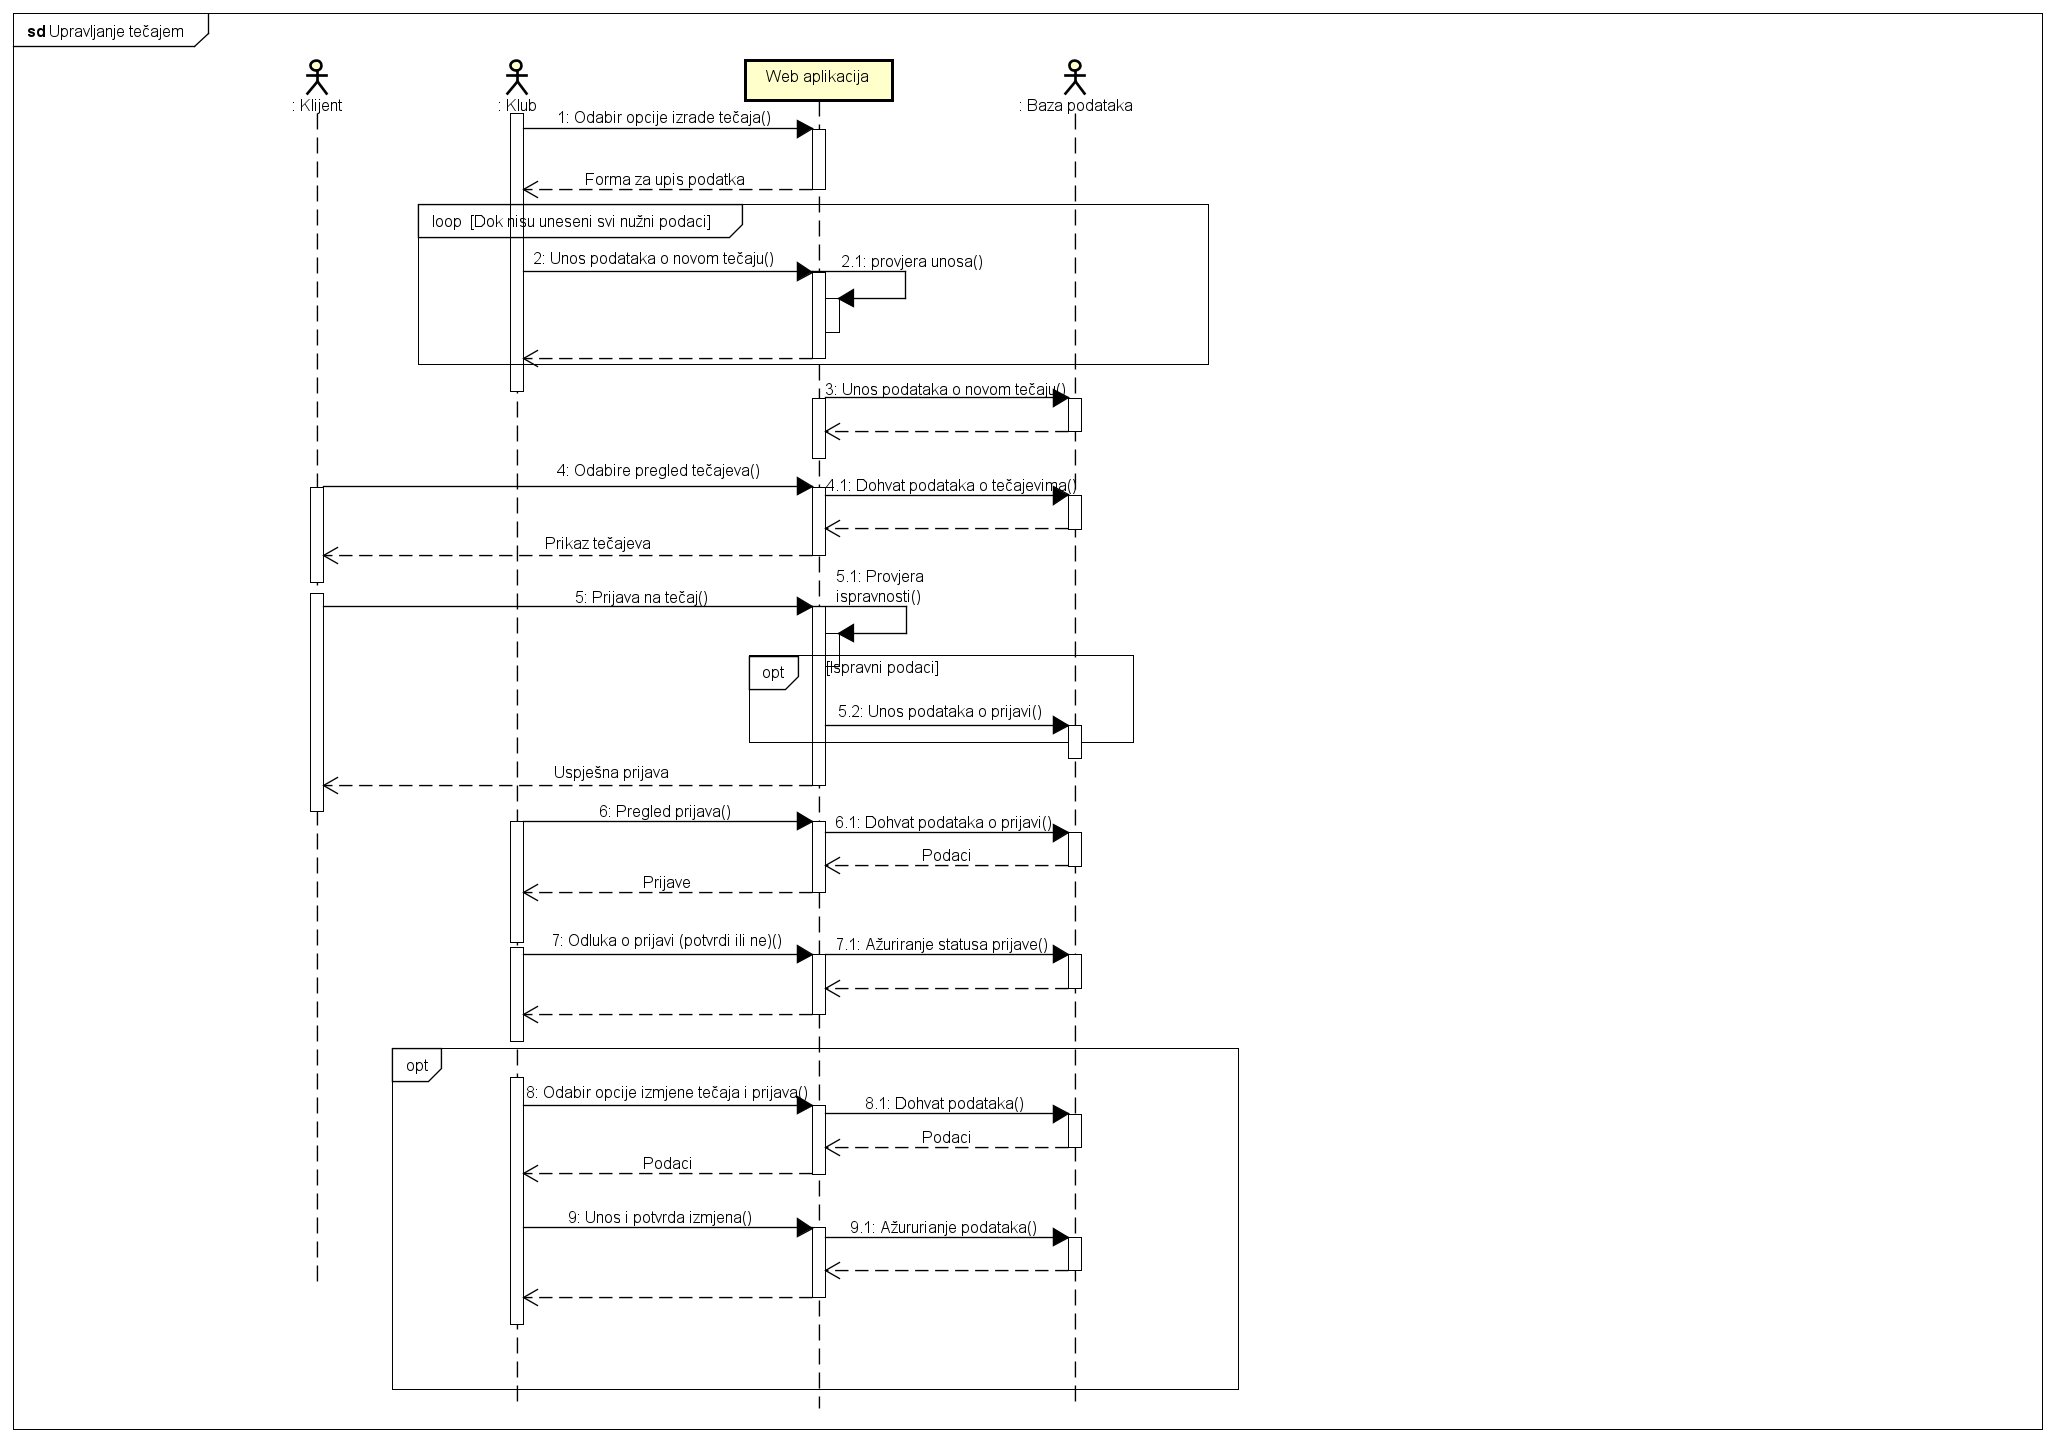
\includegraphics[scale=0.4]{slike/SD-Upravljanje tečajem.PNG} %veličina slike u odnosu na originalnu datoteku i pozicija slike
			\centering
			\caption{Sekvencijski dijagram - Dodavanje tečajeva i prijava na tečajeve}
			\label{fig:tecaj}
		\end{figure}

				\noindent \textbf {Obrasci uporabe UC6, UC7 i UC8 – dodavanje plesova, izmjena plesova i brisanje plesova }
Administrator može dodavati nove plesove i vršiti promjenu nad već postojećim plesovima. Ukoliko se administrator odluči za dodavanje plesa, on šalje poslužitelju zahtjev za stvaranje novog plesa, nakon čega web aplikacija vrši dohvat podataka iz baze te vraća administratoru formu za unos podataka. Administrator ispunjava podatke o novom plesu, a zatim poslužitelj provjerava ispravnost unesenih podataka i šalje ih u bazu podataka. Ukoliko se administrator odluči za izmjenu plesova, on šalje zahtjev poslužitelju za odabir dostupnih plesova. Poslužitelj dohvaća dostupne plesove iz baze te ih vraća poslužitelju. Poslužitelj zatim nad dostupnim plesovima vrši promjene ili briše ples, nakon čega poslužitelj pohranjuje izmjene u bazu podataka
		
		\begin{figure}[H]
			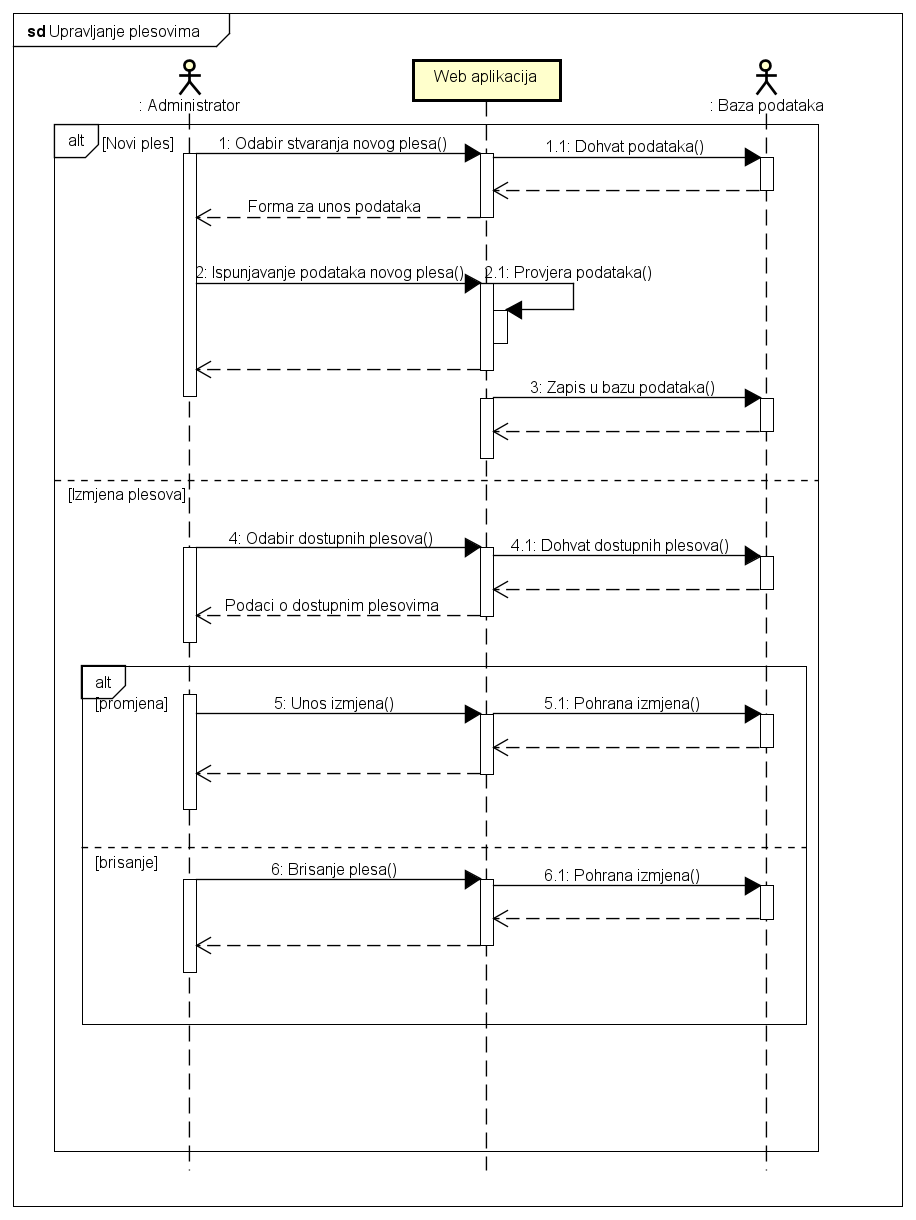
\includegraphics[scale=0.4]{slike/SD-Upravljanje plesovima.PNG} %veličina slike u odnosu na originalnu datoteku i pozicija slike
			\centering
			\caption{Sekvencijski dijagram - Dodavanje, izmjena i brisanje plesova}
			\label{fig:administr}
		\end{figure}
		

				\eject
	
		\section{Ostali zahtjevi}
	
			\begin{packed_item}
	
				\item Sustav treba omogućiti rad više korisnika u stvarnom vremenu
				\item Sustav treba ispravno funkcionirati u svim web preglednicima
				\item Korisničko sučelje i sustav moraju podržavati hrvatsku abecedu (dijakritičke znakove) pri unosu i prikazu tekstualnog sadržaja
				\item Potpuno učitavanje početne stranice aplikacije ne smije trajati duže od 3 sekunde
				\item Izvršavanje dijela programa u kojem se pristupa bazi podataka ne smije trajati duže od 4 sekunde
				\item Sustav treba biti implementiran kao web aplikacija koristeći objektno-orijentirane jezike
				\item Neispravno korištenje korisničkog sučelja ne smije narušiti funkcionalnost i rad sustava
				\item Sustav treba biti jednostavan za korištenje, jasan korisnicima s manje informatičkog iskustva bez opširnih uputa
				\item Nadogradnja sustava ne smije narušavati postojeće funkcionalnosti sustava
				\item Veza s bazom podataka mora biti kvalitetno zaštićena, brza i otporna na vanjske greške
				\item Sustav ne smije omogućiti registraciju korisnika dok nije unesena jaka lozinka (barem jedno veliko slovo, znamenka i specijalni znak)
				\item Sustav koristi srednjoeuropsko standardno vrijeme, GMT+1 
				\item Pristup sustavu mora biti omogućen iz javne mreže pomoću HTTPS
			\end{packed_item}
			 
			 
			 
	